\documentclass[12pt]{article}
\usepackage{geometry}                % See geometry.pdf to learn the layout options. There are lots.
\geometry{letterpaper}                   % ... or a4paper or a5paper or ... 
%\geometry{landscape}                % Activate for for rotated page geometry
\usepackage[parfill]{parskip}    % Activate to begin paragraphs with an empty line rather than an indent
\usepackage{daves,fancyhdr,natbib,graphicx,dcolumn,amsmath,lastpage,url}
\usepackage{amsmath,amssymb,epstopdf,longtable}
\usepackage{paralist} 
\DeclareGraphicsRule{.tif}{png}{.png}{`convert #1 `dirname #1`/`basename #1 .tif`.png}
\pagestyle{fancy}
\lhead{CE 3372 -- Water Systems Design}
\rhead{SPRING 2025}
\lfoot{EXERCISE 3}
\cfoot{}
\rfoot{Page \thepage\ of \pageref{LastPage}}
\renewcommand\headrulewidth{0pt}

\begin{document}
\begin{center}
{\textbf{{ CE 3372 -- Water Systems Design} \\ {Demand Estimation} \\ {Exercise Set 3}}}
\end{center}

\section*{\small{Exercise}} 
\begin{enumerate}
%\item %Figure \ref{fig:newport-base-map} is a map of a proposed subdivision.  Each lot will house an executive home.  

%\begin{figure}[h!] %  figure placement: here, top, bottom, or page
%\centering
%   \includegraphics[width=6in]{newport-base-map.jpg}
%   \caption{Newport Subdivision Proposed Development}
%   \label{fig:newport-base-map} 
%\end{figure}
%\clearpage



%Figure \ref{fig:newport-pipe-layout} is a skeletonized layout for a network model of the water distribution system.
%Each small black circle is a distribution node that serves several lots.
%Each red circle represents a fire-hydrant location.
%Water is supplied by the lift station depicted in the lower left corner of the drawing.   
%
%\begin{enumerate}[a)]
%\item Estimate the average daily demand (ADD) for the entire distribution system using San Marcos, Texas water system design guidelines.
%\item Estimate the maximum daily demand (MDD) for the entire distribution system using San Marcos, Texas water system design guidelines.
%\item Estimate the maximum daily demand (MDD) + fire flow for the entire distribution system using San Marcos, Texas water system design guidelines.
%\item Estimate the peak hourly demand (PHD) for the entire distribution system using San Marcos, Texas water system design guidelines.
%\item Estimate the average daily demand (ADD) for the entire distribution system using Riverside County, CA. water system design guidelines.
%\item Estimate the maximum daily demand (MDD) for the entire distribution system using Riverside County, CA. water system design guidelines.
%\item Estimate the maximum daily demand (MDD) + fire flow for the entire distribution system using Riverside County, CA. water system design guidelines.
%\item Estimate the peak hourly demand (PHD) for the entire distribution system using Riverside County, CA. water system design guidelines.
%\end{enumerate}
%
%\begin{figure}[h!] %  figure placement: here, top, bottom, or page
%\centering
%   \includegraphics[width=6in]{newport-pipe-layout-flat.png}
%   \caption{Newport Subdivision EPANET Model Pipe Layout}
%   \label{fig:newport-pipe-layout} 
%\end{figure}
%\clearpage
\item Figure \ref{fig:water_network_layout} is a layout of a hydraulic network model for the Somewhere USA subdivision.   
The blue line segments are pipes and are labeled (P1, P2, $\dots$).   
The blue circles are nodes and are labeled (N1, N2, $\dots$).
The yellow polygons represent the lots assigned to each node; for example, node N2 supplies the six (6) lots located near the node.
\begin{figure}[ht!] %  figure placement: here, top, bottom, or page
   \centering
   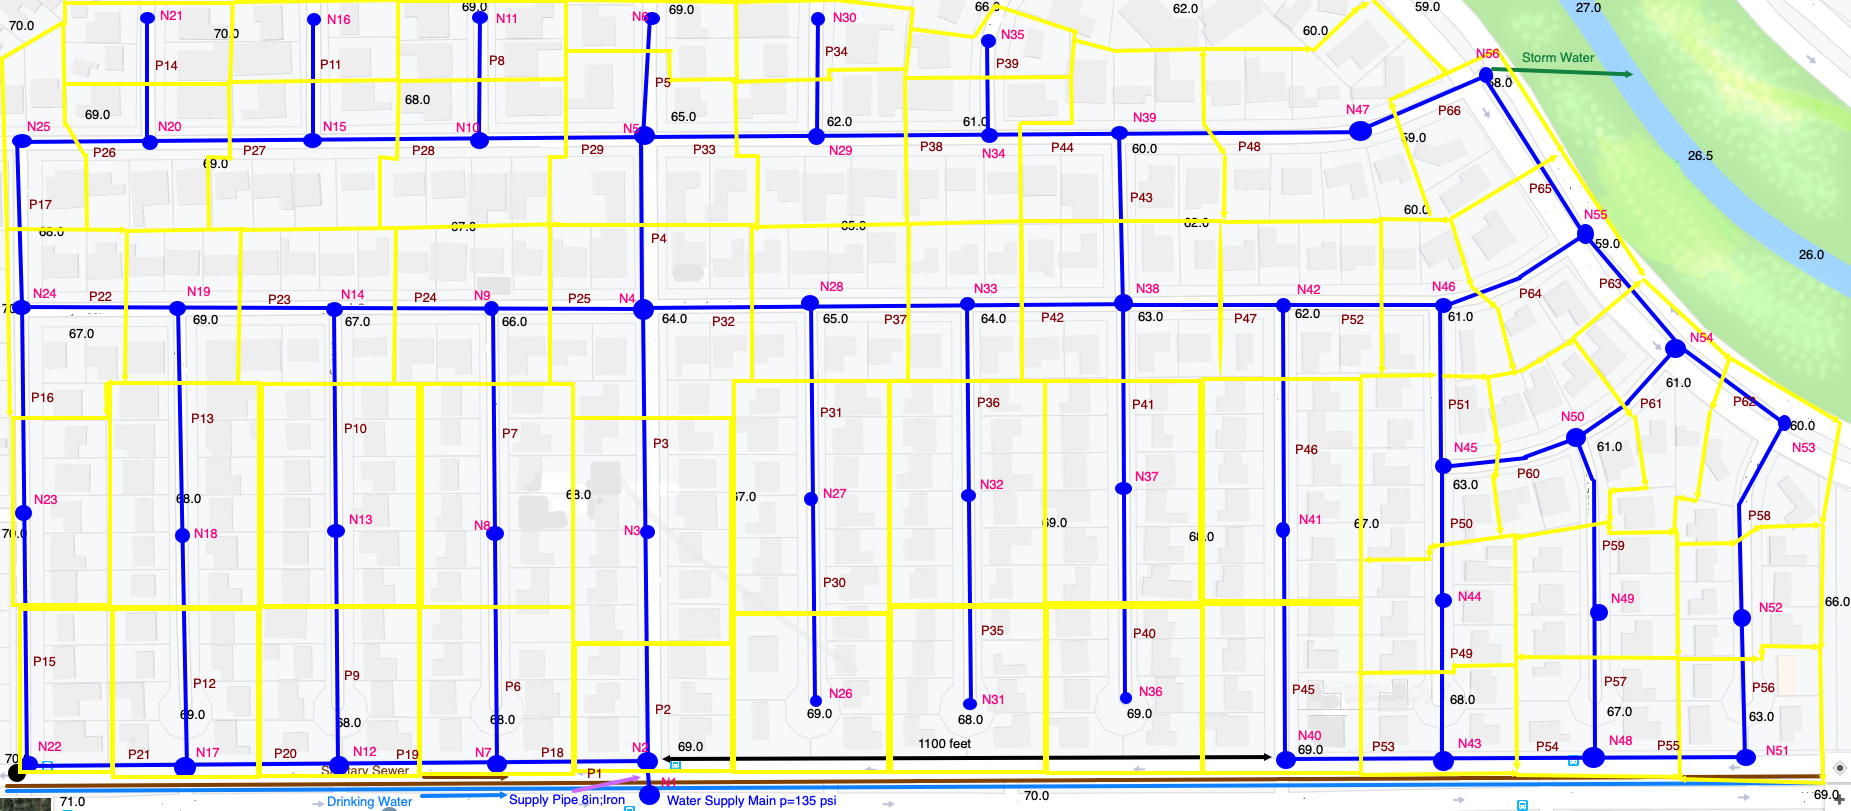
\includegraphics[width=6.5in]{SomewhereClipNodes.jpg} 
   \caption{Hydraulic Model Network for Somewhere USA}
   \label{fig:water_network_layout}
\end{figure}
\begin{enumerate}[a)]
\item Determine the number of lots served by each node, these will constitute the by-node service unit equivalent (SUE).

This estimate is simply a matter of counting the "houses" depicted in the drawing. I counted 355 lots - your values will be close (they should be the same, but I imagine there will be some variation but only a few lots)

\item Estimate the average daily demand (ADD), by-node, for distribution system using San Marcos, Texas water system design guidelines.

This estmate uses guidance in Figure \ref{fig:hydrant0}, which is 0.24 gpm/SUE

\item Estimate the maximum daily demand (MDD), by-node, for the distribution system using San Marcos, Texas water system design guidelines.

This estmate uses guidance in Figure \ref{fig:hydrant0}, which is 0.70 gpm/SUE

\item Estimate the maximum daily demand (MDD) + fire flow, by-node for the distribution system using San Marcos, Texas water system design guidelines.

This estimate requires locating fire hydrants on the drawing (not supplied).  For simplicity in planning apply the following parts of the San Marcos manual:

First consider flow per hydrant - it is unlikely the whole area will be on fire at once (unless it is in Los Angeles in January 2025) but a decent worst case would be 1000 gpm/hydrant (which should nicely oversize a system).  The alternative is to find the ISO standards that are appliciable and use them, but the supplied information is pretty sparse for this application.

\begin{figure}[h!] %  figure placement: here, top, bottom, or page
   \centering
   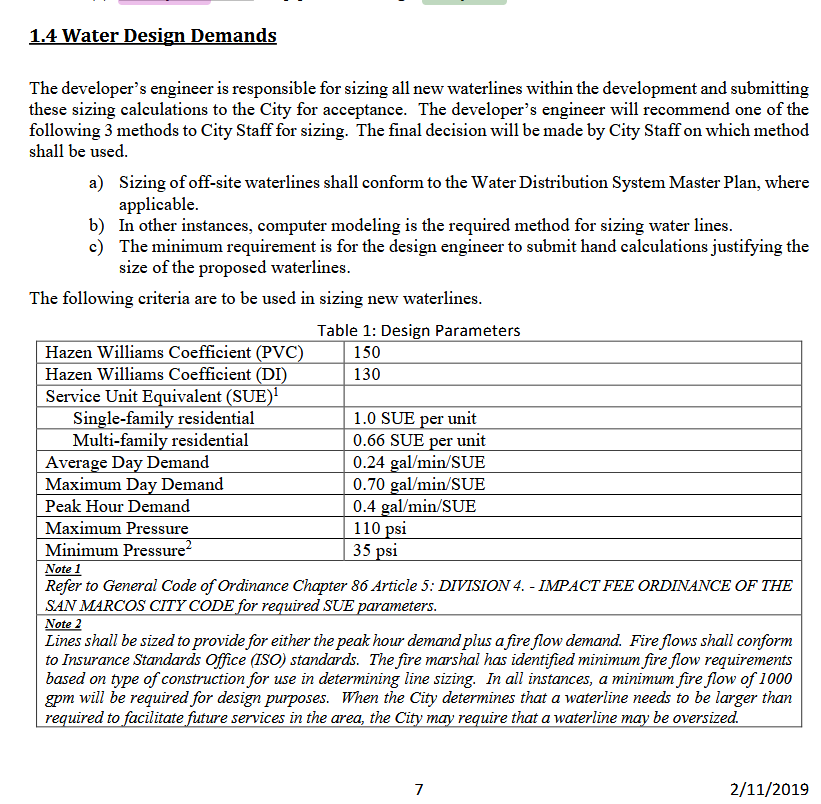
\includegraphics[width=5.5in]{Hydrants-0.png} 
   \caption{Fire Flow guidelines - here we interpret as 1000 gpm/hydrant as a conservative value}
   \label{fig:hydrant0}
\end{figure}

\clearpage

Our next part is to determine the hydrant locations (for a demand estimate - actual locations are more complex).   In the same manual a spacing specification states that all parts of the area should be within 500 feet of a hydrant (using a Manhattan distance definition, which is not the same as the usual cartesian distance we usually use).

\begin{figure}[h!] %  figure placement: here, top, bottom, or page
   \centering
   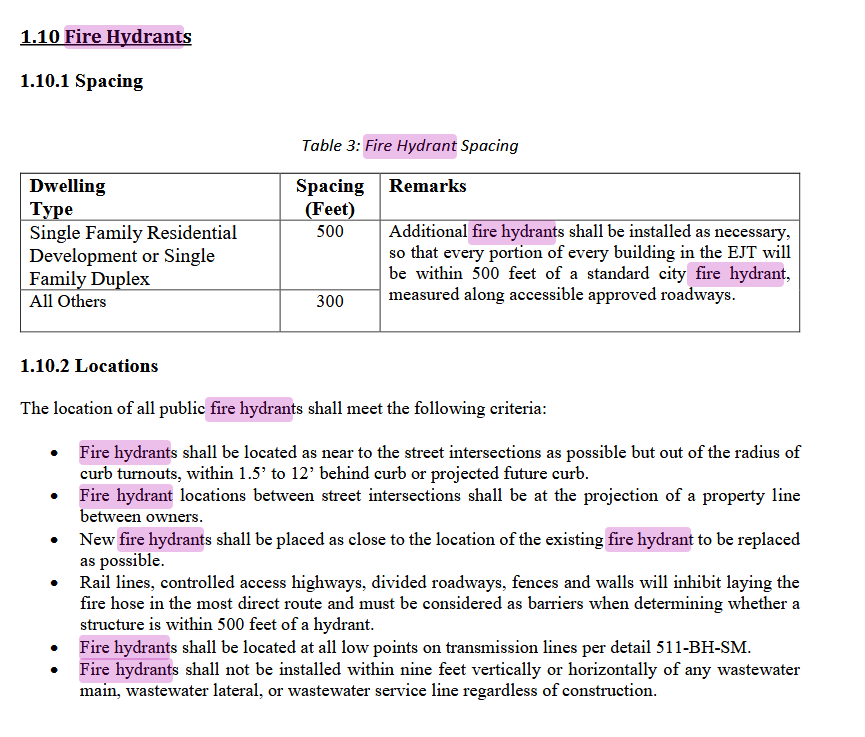
\includegraphics[width=5.5in]{Hydrants-1.png} 
   \caption{Fire Hydrant spacing guidelines}
   \label{fig:hydrant1}
\end{figure}
\clearpage

Using the spacing guidelines (and some practical judgement on how hard it might be to drag a firehose 500 feet we can identify hydrant locations for the purpose of estimating demand.

\begin{figure}[h!] %  figure placement: here, top, bottom, or page
   \centering
   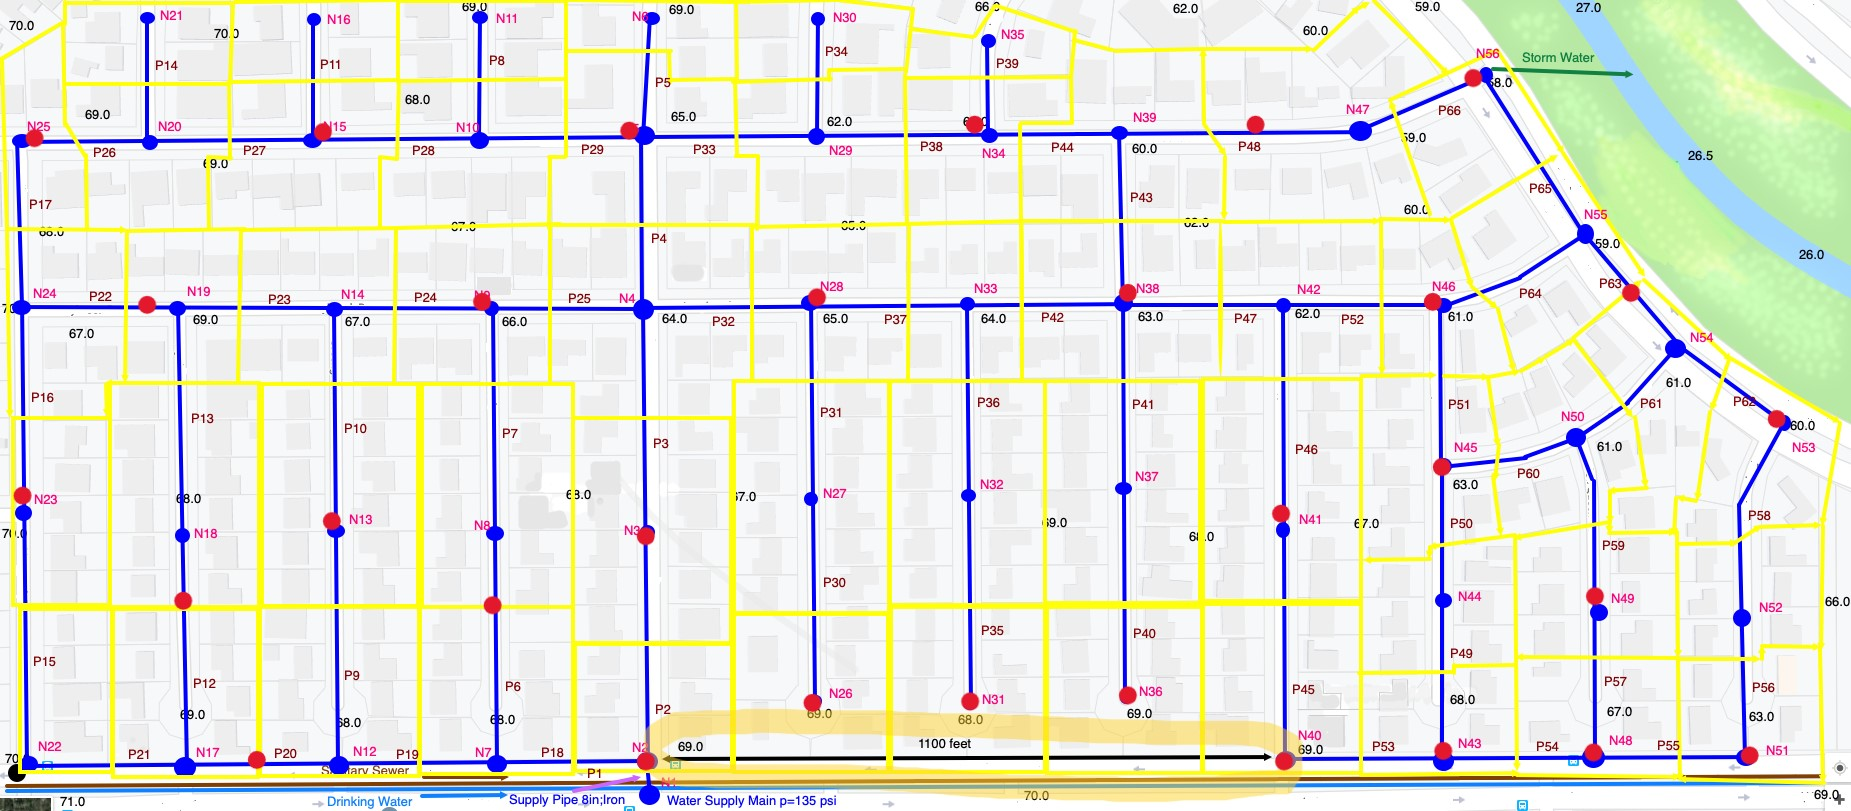
\includegraphics[width=6.5in]{SomewhereHydrants.jpg} 
   \caption{Hydrant locations (for fire flow estimation)}
   \label{fig:water_network_layout}
\end{figure}

The few hydrants not colocated with a node would be either assigned to the nearest node or distributed to the two nearest nodes.  I choose the later approach.
\clearpage

\item Estimate the peak hourly demand (PHD), by-node, for the distribution system using San Marcos, Texas water system design guidelines.

This estmate uses guidance in Figure \ref{fig:hydrant0}, which is 0.40 gpm/SUE
\end{enumerate}

Use your estimates to produce a completed version of Table \ref{tab:ByNodes}.
Save the table (in a file) -- you will need it later in another homework problem.

% Requires the booktabs if the memoir class is not being used
\begin{table}[h!]
   \centering
   \caption{Node Demands for Somewhere USA Distribution System}
   \begin{tabular}{p{0.5in}p{0.7in}p{0.7in}p{0.7in}p{0.7in}p{0.8in}p{0.7in}} % Column formatting, @{} suppresses leading/trailing space
Node & SUE & ADD & MDD & Fire & Fire+MDD & PHD \\
\hline
\hline
N1&0&~&~&~&~&\\
N2&6&1.44&4.2&1000&1004.2&2.4\\
N3&12&2.88&8.4&1000&1008.4&4.8\\
N4&10&2.4&7&&7&4.0\\
N5&5&1.2&3.5&1000&1003.5&2.0\\
N6&3&0.72&2.1&&2.1&1.2\\
N7&7&1.68&4.9&500&504.9&2.8\\
N8&12&2.88&8.4&500&508.4&4.8\\
N9&7&1.68&4.9&1000&1004.9&2.8\\
N10&6&1.44&4.2&&4.2&2.4\\
N11&4&0.96&2.8&&2.8&1.6\\
N12&8&1.92&5.6&&5.6&3.2\\
N13&12&2.88&8.4&1000&1008.4&4.8\\
N14&7&1.68&4.9&&4.9&2.8\\
N15&6&1.44&4.2&1000&1004.2&2.4\\
N16&4&0.96&2.8&&2.8&1.6\\
N17&8&1.92&5.6&1000&1005.6&3.2\\
N18&12&2.88&8.4&500&508.4&4.8\\
N19&5&1.2&3.5&1000&1003.5&2.0\\
N20&5&1.2&3.5&&3.5&2.0\\
N21&4&0.96&2.8&&2.8&1.6\\
N22&4&0.96&2.8&&2.8&1.6\\
N23&5&1.2&3.5&1000&1003.5&2.0\\
N24&5&1.2&3.5&&3.5&2.0\\
N25&3&0.72&2.1&1000&1002.1&1.2\\
N26&6&1.44&4.2&1000&1004.2&2.4\\
N27&12&2.88&8.4&&8.4&4.8\\
N28&7&1.68&4.9&1000&1004.9&2.8\\
N29&5&1.2&3.5&&3.5&2.0\\
N30&3&0.72&2.1&&2.1&1.2\\
N31&8&1.92&5.6&1000&1005.6&3.2\\
N32&12&2.88&8.4&&8.4&4.8\\
N33&5&1.2&3.5&&3.5&2.0\\
N34&5&1.2&3.5&1000&1003.5&2.0\\
N35&2&0.48&1.4&&1.4&0.8\\
   \end{tabular}

   \label{tab:ByNodes}
\end{table}

\begin{table}[h!]
   \centering
   \caption{Node Demands for Somewhere USA Distribution System (Continued)}
   \begin{tabular}{p{0.5in}p{0.7in}p{0.7in}p{0.7in}p{0.7in}p{0.8in}p{0.7in}} % Column formatting, @{} suppresses leading/trailing space
Node & SUE & ADD & MDD & Fire & Fire+MDD & PHD \\
\hline
\hline
N36&8&1.92&5.6&1000&1005.6&3.2\\
N37&12&2.88&8.4&&8.4&4.8\\
N38&8&1.92&5.6&1000&1005.6&3.2\\
N39&7&1.68&4.9&500&504.9&2.8\\
N40&8&1.92&5.6&1000&1005.6&3.2\\
N41&12&2.88&8.4&1000&1008.4&4.8\\
N42&7&1.68&4.9&&4.9&2.8\\
N43&4&0.96&2.8&1000&1002.8&1.6\\
N44&6&1.44&4.2&&4.2&2.4\\
N45&7&1.68&4.9&1000&1004.9&2.8\\
N46&4&0.96&2.8&1000&1002.8&1.6\\
N47&9&2.16&6.3&500&506.3&3.6\\
N48&4&0.96&2.8&1000&1002.8&1.6\\
N49&6&1.44&4.2&1000&1004.2&2.4\\
N50&6&1.44&4.2&&4.2&2.4\\
N51&4&0.96&2.8&1000&1002.8&1.6\\
N52&6&1.44&4.2&&4.2&2.4\\
N53&3&0.72&2.1&1000&1002.1&1.2\\
N54&4&0.96&2.8&500&502.8&1.6\\
N55&3&0.72&2.1&500&502.1&1.2\\
N56&2&0.48&1.4&1000&1001.4&0.8\\
\hline
Totals:&355&85.2&248.5&29500&29748.5&142\\
\hline
   \end{tabular}

   \label{tab:ByNodes2}
\end{table}
\clearpage
%%%%%%%%%%%%%%%%%%%%%%%%%%%%%%%%%%%%%%%%%%%%%%%%%%%%%%%
%%%%%%%%%%%%%%% PROBLEM 2 %%%%%%%%%%%%%%%%%%%%%%%%%%%%%%%%%
%%%%%%%%%%%%%%%%%%%%%%%%%%%%%%%%%%%%%%%%%%%%%%%%%%%%%%%


\end{enumerate}




\end{document}  